\documentclass{beamer}\usepackage[]{graphicx}\usepackage[]{color}
%% maxwidth is the original width if it is less than linewidth
%% otherwise use linewidth (to make sure the graphics do not exceed the margin)
\makeatletter
\def\maxwidth{ %
  \ifdim\Gin@nat@width>\linewidth
    \linewidth
  \else
    \Gin@nat@width
  \fi
}
\makeatother

\definecolor{fgcolor}{rgb}{1, 0.894, 0.769}
\newcommand{\hlnum}[1]{\textcolor[rgb]{0.824,0.412,0.118}{#1}}%
\newcommand{\hlstr}[1]{\textcolor[rgb]{1,0.894,0.71}{#1}}%
\newcommand{\hlcom}[1]{\textcolor[rgb]{0.824,0.706,0.549}{#1}}%
\newcommand{\hlopt}[1]{\textcolor[rgb]{1,0.894,0.769}{#1}}%
\newcommand{\hlstd}[1]{\textcolor[rgb]{1,0.894,0.769}{#1}}%
\newcommand{\hlkwa}[1]{\textcolor[rgb]{0.941,0.902,0.549}{#1}}%
\newcommand{\hlkwb}[1]{\textcolor[rgb]{0.804,0.776,0.451}{#1}}%
\newcommand{\hlkwc}[1]{\textcolor[rgb]{0.78,0.941,0.545}{#1}}%
\newcommand{\hlkwd}[1]{\textcolor[rgb]{1,0.78,0.769}{#1}}%
\let\hlipl\hlkwb

\usepackage{framed}
\makeatletter
\newenvironment{kframe}{%
 \def\at@end@of@kframe{}%
 \ifinner\ifhmode%
  \def\at@end@of@kframe{\end{minipage}}%
  \begin{minipage}{\columnwidth}%
 \fi\fi%
 \def\FrameCommand##1{\hskip\@totalleftmargin \hskip-\fboxsep
 \colorbox{shadecolor}{##1}\hskip-\fboxsep
     % There is no \\@totalrightmargin, so:
     \hskip-\linewidth \hskip-\@totalleftmargin \hskip\columnwidth}%
 \MakeFramed {\advance\hsize-\width
   \@totalleftmargin\z@ \linewidth\hsize
   \@setminipage}}%
 {\par\unskip\endMakeFramed%
 \at@end@of@kframe}
\makeatother

\definecolor{shadecolor}{rgb}{.97, .97, .97}
\definecolor{messagecolor}{rgb}{0, 0, 0}
\definecolor{warningcolor}{rgb}{1, 0, 1}
\definecolor{errorcolor}{rgb}{1, 0, 0}
\newenvironment{knitrout}{}{} % an empty environment to be redefined in TeX

\usepackage{alltt}
\usepackage{../371g-slides}
\title{Model Building}
\subtitle{Lecture 14}
\author{STA 371G}
\IfFileExists{upquote.sty}{\usepackage{upquote}}{}
\begin{document}
  
  

  \frame{\maketitle}

  % Show outline at beginning of each section
  \AtBeginSection[]{ 
    \begin{frame}<beamer>
      \tableofcontents[currentsection]
    \end{frame}
  }

  %%%%%%% Slides start here %%%%%%%

  \begin{darkframes}
    
    
    \begin{frame}{There is a Primary Care Physician Shortage in Texas!}
      \begin{center}
        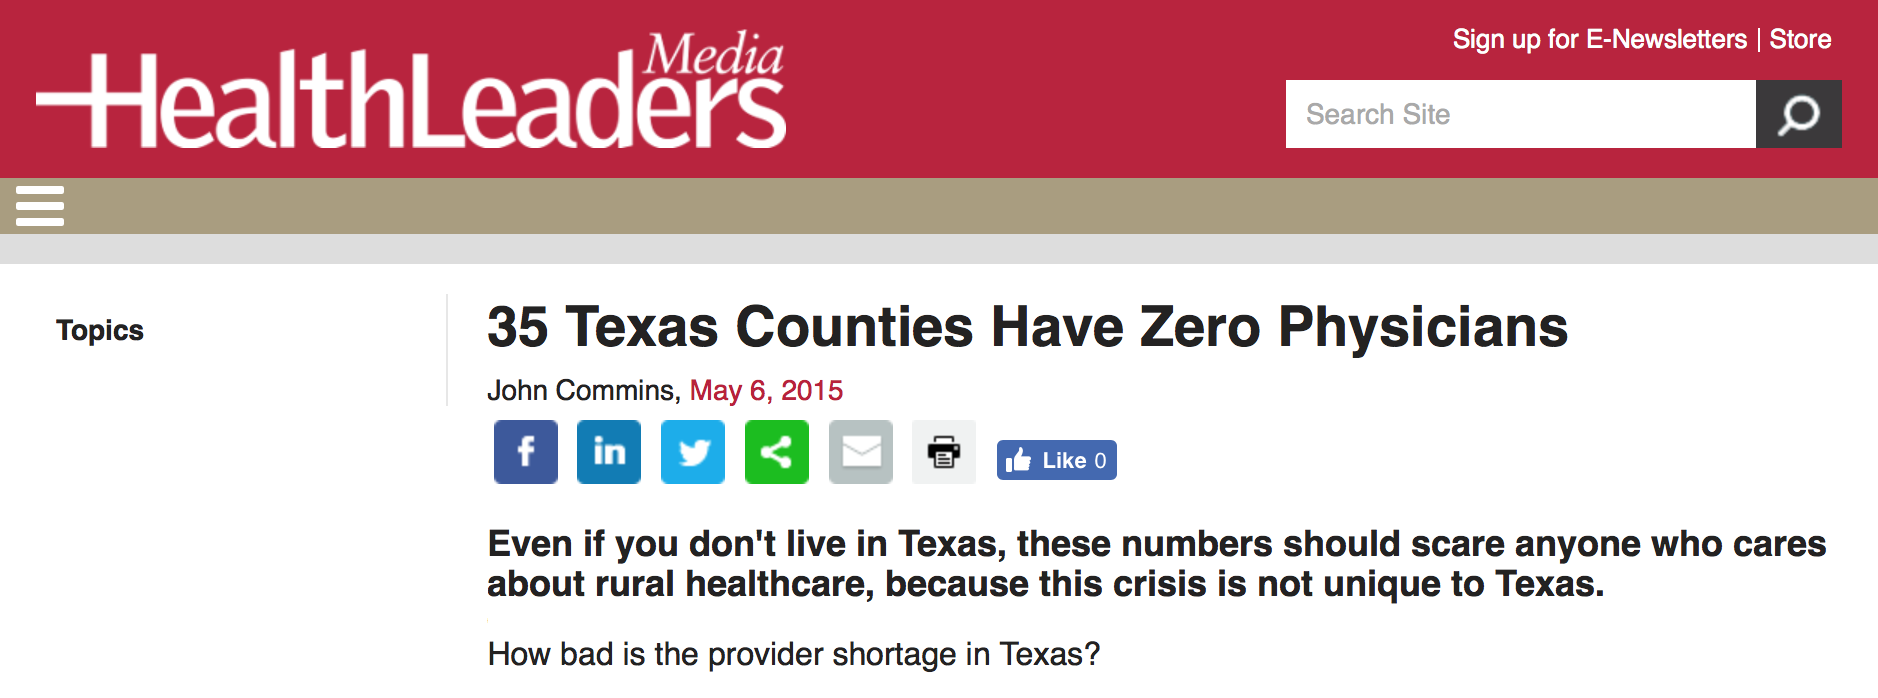
\includegraphics[width=3.8in]{DocShortage} \\
      \end{center} \pause

      \begin{center}
        {What might explain this? There are many potential predictors!}
      \end{center} 

      \begin{columns}[onlytextwidth]
        \column{.5\textwidth} 
          \begin{itemize}
            \item Small counties
            \item Poverty
            \item Health insurance
          \end{itemize}
        \column{.5\textwidth}
          \begin{itemize}
            \item Unemployment
            \item Large rural areas
            \item Something else?
          \end{itemize}
      \end{columns}
      
      \lc {smallest population}
    \end{frame}

    \begin{frame}[fragile]{What to do if there a lot of potential predictors}
      \begin{itemize}[<+->]
        \item Previously, we assumed that the explanatory variables were either from a small set or chosen in advance.
        \item However, selecting the explanatory variables, or figuring out what predicts the number of physicians that a county has, is a large part of the analysis in this case.
        \item This type of analysis is an exploratory study.
      \end{itemize} 
    \end{frame}

    \begin{frame}[fragile]{An exploratory study of the Texas physician shortage}
      \begin{itemize}[<+->]
        \item Exploratory studies are observational studies, in that the variables are observed rather than controlled, which is different from an experiment.
        \item Multicollinearity is much more likely in an exploratory study than in an experiment or a confirmatory study.
        \item Exploratory studies require the most in terms of model selection. Automated tools are helpful, but judgement is still needed!
      \end{itemize} 
    \end{frame}

    \begin{frame}[fragile]{Population as a predictor of number of physicians}
          
\begin{knitrout}
\definecolor{shadecolor}{rgb}{0.137, 0.137, 0.137}\begin{kframe}
\begin{alltt}
\hlkwd{plot}\hlstd{(counties}\hlopt{$}\hlstd{Population, counties}\hlopt{$}\hlstd{Physicians)}
\hlstd{popmodel} \hlkwb{<-} \hlkwd{lm}\hlstd{(counties}\hlopt{$}\hlstd{Physicians} \hlopt{~} \hlstd{counties}\hlopt{$}\hlstd{Population)}
\hlkwd{abline}\hlstd{(popmodel)}
\end{alltt}
\end{kframe}
% Created by tikzDevice version 0.10.1 on 2017-03-08 21:07:53
% !TEX encoding = UTF-8 Unicode


\end{knitrout}

      \lc {What is R2  If we predict}
    \end{frame}

    \begin{frame}[fragile]{Transform and Subset the data}

\begin{knitrout}
\definecolor{shadecolor}{rgb}{0.137, 0.137, 0.137}\begin{kframe}
\begin{alltt}
\hlcom{# Transform Physians}
\hlstd{counties}\hlopt{$}\hlstd{PhysiciansPer10000} \hlkwb{<-}
     \hlstd{(counties}\hlopt{$}\hlstd{Physicians}\hlopt{/}\hlstd{counties}\hlopt{$}\hlstd{Population)}\hlopt{*}\hlnum{10000}

\hlcom{# Remove the very small and very large counties}
\hlstd{mcounties} \hlkwb{<-} \hlstd{counties[counties}\hlopt{$}\hlstd{Population} \hlopt{<} \hlnum{500000} \hlopt{&}
                      \hlstd{counties}\hlopt{$}\hlstd{Population} \hlopt{>} \hlnum{10000}\hlstd{,]}

\hlcom{# Show medium counties with no physicians}
\hlstd{mcounties[mcounties}\hlopt{$}\hlstd{Physicians} \hlopt{==} \hlnum{0}\hlstd{,} \hlkwd{c}\hlstd{(}\hlnum{1}\hlstd{,}\hlnum{5}\hlstd{,}\hlnum{12}\hlstd{)]}
\end{alltt}
\begin{verbatim}
      X MedianIncome PctUnemployed
157 157        51481           3.5
159 159        35069           5.5
\end{verbatim}
\end{kframe}
\end{knitrout}

        \lc {Why would we want to remove}
    \end{frame}

    \begin{frame}[fragile]{The 10 potential x variables}
          \begin{itemize}
            \item LandArea:       Area in quare miles
            \item PctRural:       Percentage rural land
            \item MedianIncome:   Median household income
            \item Population:     Population
            \item PctUnder18:     Percent children
            \item PctOver65:      Percent seniors
            \item PctPoverty:     Percent below the poverty line
            \item PctUninsured:   Percent without health insurance
            \item PctSomeCollege: Percent with some higher education
            \item PctUnemployed:  Percent unemployed
          \end{itemize}
    \end{frame}

    \begin{frame}[fragile]{Building all of the possible models}
      \begin{itemize}[<+->]
        \item Previously, we built the full model and eliminated the variables in order of largest p-value (or smallest t-score). This is what the reading assignment calls backward stepwise regression.
        \item This method is not guaranteed to find to the best model!
        \item If there are n candidate predictor variables, there are $2^n$ possible models, and we need to look at ALL of them to be sure that we have found the best model.
        \item This is where R's automated model building tools help.
      \end{itemize} 
    \end{frame}

    \begin{frame}[fragile]{How to decide which model is best}
      \begin{itemize}[<+->]
        \item We have used $R^2$ and Adjusted-$R^2$ to select the best models
        \item But $R^2$ is not good for comparing models with differnet numbers of variables because it tends to increase a little bit with each additional variable just due to randomness.
        \item Adjusted-$R^2$ is better because it multiplies $R^2$ by a penalty that depends on the number of variables, but the penalty is somewhat arbitrary and increases as the number of variables increases.
      \end{itemize} 
    \end{frame}


    \begin{frame}[fragile]{There are many ways to decide which model is best}
      \begin{itemize}[<+->]
        \item All model measuring criteria try to find a balance between the predictive power of the model and the number of variables.
        \item No method is ideal in all situations, so it is generally best to use multiple methods and look at the results.
        \item AIC (Akaike’s Information Criterion) and the very similar BIC (your reading calls it SBC) are other widely used criterion that often gives different results than Adjusted-$R^2$.
      \end{itemize} 

      \lc  
    \end{frame}  

    \begin{frame}[fragile]{Stepping forwards}

       The step() function uses the AIC criterion to compare models. You must build the null and the full models first.

\begin{knitrout}
\definecolor{shadecolor}{rgb}{0.137, 0.137, 0.137}\begin{kframe}
\begin{alltt}
\hlstd{null} \hlkwb{<-} \hlkwd{lm}\hlstd{(PhysiciansPer10000}\hlopt{~}\hlnum{1}\hlstd{,} \hlkwc{data}\hlstd{=mcounties)}

\hlstd{full} \hlkwb{<-} \hlkwd{lm}\hlstd{(PhysiciansPer10000} \hlopt{~} \hlstd{LandArea}\hlopt{+}\hlstd{PctRural}\hlopt{+}
           \hlstd{MedianIncome}\hlopt{+}\hlstd{Population}\hlopt{+}\hlstd{PctUnder18}\hlopt{+}
           \hlstd{PctOver65}\hlopt{+}\hlstd{PctPoverty}\hlopt{+}\hlstd{PctUninsured}\hlopt{+}
           \hlstd{PctSomeCollege}\hlopt{+}\hlstd{PctUnemployed,} \hlkwc{data}\hlstd{=mcounties)}

\hlstd{stepforward.out} \hlkwb{<-} \hlkwd{step}\hlstd{(null,} \hlkwc{scope}\hlstd{=}\hlkwd{list}\hlstd{(}\hlkwc{lower}\hlstd{=null,} \hlkwc{upper}\hlstd{=full),}
                              \hlkwc{direction} \hlstd{=}\hlstr{"forward"}\hlstd{)}
\end{alltt}
\begin{verbatim}
Start:  AIC=238.65
PhysiciansPer10000 ~ 1

                 Df Sum of Sq    RSS    AIC
+ PctSomeCollege  1   150.125 558.67 203.28
+ Population      1   132.562 576.23 208.14
+ PctRural        1   119.850 588.94 211.57
+ PctUnemployed   1    32.121 676.67 233.37
+ MedianIncome    1    30.413 678.38 233.76
+ PctPoverty      1    14.337 694.45 237.44
<none>                        708.79 238.65
+ PctUnder18      1     2.503 706.29 240.09
+ LandArea        1     2.260 706.53 240.15
+ PctOver65       1     0.463 708.33 240.55
+ PctUninsured    1     0.374 708.42 240.57

Step:  AIC=203.28
PhysiciansPer10000 ~ PctSomeCollege

                Df Sum of Sq    RSS    AIC
+ PctRural       1    65.200 493.47 185.80
+ Population     1    39.046 519.62 193.91
<none>                       558.67 203.28
+ PctUnemployed  1     6.141 552.53 203.55
+ MedianIncome   1     4.967 553.70 203.88
+ PctPoverty     1     2.469 556.20 204.59
+ PctOver65      1     2.204 556.46 204.66
+ PctUninsured   1     1.338 557.33 204.91
+ PctUnder18     1     1.138 557.53 204.96
+ LandArea       1     1.113 557.55 204.97

Step:  AIC=185.8
PhysiciansPer10000 ~ PctSomeCollege + PctRural

                Df Sum of Sq    RSS    AIC
+ PctOver65      1    71.210 422.26 163.33
+ PctUnder18     1    43.408 450.06 173.34
+ Population     1     8.265 485.20 185.15
<none>                       493.47 185.80
+ PctUnemployed  1     5.721 487.75 185.97
+ MedianIncome   1     4.008 489.46 186.52
+ PctUninsured   1     2.463 491.00 187.01
+ PctPoverty     1     0.985 492.48 187.48
+ LandArea       1     0.805 492.66 187.54

Step:  AIC=163.33
PhysiciansPer10000 ~ PctSomeCollege + PctRural + PctOver65

                Df Sum of Sq    RSS    AIC
+ Population     1   23.8333 398.42 156.21
+ PctUnder18     1    7.6234 414.63 162.47
+ PctUnemployed  1    6.4549 415.80 162.91
+ PctUninsured   1    5.7792 416.48 163.17
<none>                       422.26 163.33
+ PctPoverty     1    0.1451 422.11 165.28
+ MedianIncome   1    0.0296 422.23 165.32
+ LandArea       1    0.0207 422.24 165.32

Step:  AIC=156.21
PhysiciansPer10000 ~ PctSomeCollege + PctRural + PctOver65 + 
    Population

                Df Sum of Sq    RSS    AIC
+ PctUnemployed  1   12.4148 386.01 153.24
+ PctUninsured   1    8.2151 390.21 154.94
+ PctUnder18     1    5.8479 392.58 155.89
<none>                       398.42 156.21
+ PctPoverty     1    0.8309 397.59 157.88
+ MedianIncome   1    0.1882 398.24 158.13
+ LandArea       1    0.0257 398.40 158.20

Step:  AIC=153.24
PhysiciansPer10000 ~ PctSomeCollege + PctRural + PctOver65 + 
    Population + PctUnemployed

               Df Sum of Sq    RSS    AIC
+ PctUninsured  1    6.6717 379.34 152.50
<none>                      386.01 153.24
+ PctUnder18    1    3.9987 382.01 153.60
+ MedianIncome  1    1.3362 384.67 154.69
+ PctPoverty    1    0.8056 385.20 154.91
+ LandArea      1    0.3540 385.65 155.09

Step:  AIC=152.5
PhysiciansPer10000 ~ PctSomeCollege + PctRural + PctOver65 + 
    Population + PctUnemployed + PctUninsured

               Df Sum of Sq    RSS    AIC
<none>                      379.34 152.50
+ PctUnder18    1   2.73293 376.60 153.37
+ MedianIncome  1   0.56108 378.78 154.27
+ PctPoverty    1   0.50007 378.84 154.29
+ LandArea      1   0.32092 379.02 154.37
\end{verbatim}
\end{kframe}
\end{knitrout}

      \lc 
    \end{frame}

  
    \begin{frame}[fragile]{Stepping backwards and both ways}

    You can also step backward or on both directions

\begin{knitrout}
\definecolor{shadecolor}{rgb}{0.137, 0.137, 0.137}\begin{kframe}
\begin{alltt}
\hlstd{stepbackward.out} \hlkwb{<-}
    \hlkwd{step}\hlstd{(null,} \hlkwc{scope}\hlstd{=}\hlkwd{list}\hlstd{(}\hlkwc{lower}\hlstd{=null,} \hlkwc{upper}\hlstd{=full),}
         \hlkwc{direction} \hlstd{=}\hlstr{"backward"}\hlstd{)}
\end{alltt}
\begin{verbatim}
Start:  AIC=238.65
PhysiciansPer10000 ~ 1
\end{verbatim}
\begin{alltt}
\hlstd{stepboth.out} \hlkwb{<-}
    \hlkwd{step}\hlstd{(null,} \hlkwc{scope}\hlstd{=}\hlkwd{list}\hlstd{(}\hlkwc{lower}\hlstd{=null,} \hlkwc{upper}\hlstd{=full),}
         \hlkwc{direction} \hlstd{=}\hlstr{"both"}\hlstd{)}
\end{alltt}
\begin{verbatim}
Start:  AIC=238.65
PhysiciansPer10000 ~ 1

                 Df Sum of Sq    RSS    AIC
+ PctSomeCollege  1   150.125 558.67 203.28
+ Population      1   132.562 576.23 208.14
+ PctRural        1   119.850 588.94 211.57
+ PctUnemployed   1    32.121 676.67 233.37
+ MedianIncome    1    30.413 678.38 233.76
+ PctPoverty      1    14.337 694.45 237.44
<none>                        708.79 238.65
+ PctUnder18      1     2.503 706.29 240.09
+ LandArea        1     2.260 706.53 240.15
+ PctOver65       1     0.463 708.33 240.55
+ PctUninsured    1     0.374 708.42 240.57

Step:  AIC=203.28
PhysiciansPer10000 ~ PctSomeCollege

                 Df Sum of Sq    RSS    AIC
+ PctRural        1    65.200 493.47 185.80
+ Population      1    39.046 519.62 193.91
<none>                        558.67 203.28
+ PctUnemployed   1     6.141 552.53 203.55
+ MedianIncome    1     4.967 553.70 203.88
+ PctPoverty      1     2.469 556.20 204.59
+ PctOver65       1     2.204 556.46 204.66
+ PctUninsured    1     1.338 557.33 204.91
+ PctUnder18      1     1.138 557.53 204.96
+ LandArea        1     1.113 557.55 204.97
- PctSomeCollege  1   150.125 708.79 238.65

Step:  AIC=185.8
PhysiciansPer10000 ~ PctSomeCollege + PctRural

                 Df Sum of Sq    RSS    AIC
+ PctOver65       1    71.210 422.26 163.33
+ PctUnder18      1    43.408 450.06 173.34
+ Population      1     8.265 485.20 185.15
<none>                        493.47 185.80
+ PctUnemployed   1     5.721 487.75 185.97
+ MedianIncome    1     4.008 489.46 186.52
+ PctUninsured    1     2.463 491.00 187.01
+ PctPoverty      1     0.985 492.48 187.48
+ LandArea        1     0.805 492.66 187.54
- PctRural        1    65.200 558.67 203.28
- PctSomeCollege  1    95.475 588.94 211.57

Step:  AIC=163.33
PhysiciansPer10000 ~ PctSomeCollege + PctRural + PctOver65

                 Df Sum of Sq    RSS    AIC
+ Population      1    23.833 398.42 156.21
+ PctUnder18      1     7.623 414.63 162.47
+ PctUnemployed   1     6.455 415.80 162.91
+ PctUninsured    1     5.779 416.48 163.17
<none>                        422.26 163.33
+ PctPoverty      1     0.145 422.11 165.28
+ MedianIncome    1     0.030 422.23 165.32
+ LandArea        1     0.021 422.24 165.32
- PctOver65       1    71.210 493.47 185.80
- PctSomeCollege  1    74.640 496.90 186.88
- PctRural        1   134.205 556.46 204.66

Step:  AIC=156.21
PhysiciansPer10000 ~ PctSomeCollege + PctRural + PctOver65 + 
    Population

                 Df Sum of Sq    RSS    AIC
+ PctUnemployed   1    12.415 386.01 153.24
+ PctUninsured    1     8.215 390.21 154.94
+ PctUnder18      1     5.848 392.58 155.89
<none>                        398.42 156.21
+ PctPoverty      1     0.831 397.59 157.88
+ MedianIncome    1     0.188 398.24 158.13
+ LandArea        1     0.026 398.40 158.20
- Population      1    23.833 422.26 163.33
- PctSomeCollege  1    28.714 427.14 165.13
- PctOver65       1    86.778 485.20 185.15
- PctRural        1    98.797 497.22 188.99

Step:  AIC=153.24
PhysiciansPer10000 ~ PctSomeCollege + PctRural + PctOver65 + 
    Population + PctUnemployed

                 Df Sum of Sq    RSS    AIC
+ PctUninsured    1     6.672 379.34 152.50
<none>                        386.01 153.24
+ PctUnder18      1     3.999 382.01 153.60
+ MedianIncome    1     1.336 384.67 154.69
+ PctPoverty      1     0.806 385.20 154.91
+ LandArea        1     0.354 385.65 155.09
- PctUnemployed   1    12.415 398.42 156.21
- PctSomeCollege  1    15.910 401.92 157.58
- Population      1    29.793 415.80 162.91
- PctOver65       1    90.452 476.46 184.29
- PctRural        1    95.349 481.36 185.90

Step:  AIC=152.5
PhysiciansPer10000 ~ PctSomeCollege + PctRural + PctOver65 + 
    Population + PctUnemployed + PctUninsured

                 Df Sum of Sq    RSS    AIC
<none>                        379.34 152.50
- PctUninsured    1     6.672 386.01 153.24
+ PctUnder18      1     2.733 376.60 153.37
+ MedianIncome    1     0.561 378.78 154.27
+ PctPoverty      1     0.500 378.84 154.29
+ LandArea        1     0.321 379.02 154.37
- PctUnemployed   1    10.871 390.21 154.94
- PctSomeCollege  1    15.903 395.24 156.95
- Population      1    31.780 411.12 163.13
- PctOver65       1    94.843 474.18 185.54
- PctRural        1    98.749 478.09 186.83
\end{verbatim}
\end{kframe}
\end{knitrout}

      \lc
    \end{frame}


    \begin{frame}[fragile]{Check the LINE assumptions}
      \fontsize{9}{9}\selectfont

\begin{knitrout}
\definecolor{shadecolor}{rgb}{0.137, 0.137, 0.137}\begin{kframe}
\begin{alltt}
\hlkwd{plot}\hlstd{(stepforward.out)}
\end{alltt}
\end{kframe}
% Created by tikzDevice version 0.10.1 on 2017-03-09 02:37:31
% !TEX encoding = UTF-8 Unicode

\begin{tikzpicture}[x=1pt,y=1pt]
\definecolor{fillColor}{RGB}{255,255,255}
\path[use as bounding box,fill=fillColor,fill opacity=0.00] (0,0) rectangle (289.08,216.81);
\begin{scope}
\path[clip] (  0.00,  0.00) rectangle (289.08,216.81);
\definecolor{drawColor}{RGB}{254,254,254}

\path[draw=drawColor,line width= 0.4pt,line join=round,line cap=round] ( 61.20, 85.20) --
	(251.88, 85.20) --
	(251.88,143.61) --
	( 61.20,143.61) --
	( 61.20, 85.20);
\end{scope}
\begin{scope}
\path[clip] (  0.00,  0.00) rectangle (289.08,216.81);
\definecolor{drawColor}{RGB}{254,254,254}

\node[text=drawColor,rotate= 90.00,anchor=base,inner sep=0pt, outer sep=0pt, scale=  1.00] at ( 22.80,114.40) {adjr2};
\end{scope}
\begin{scope}
\path[clip] ( 61.20, 85.20) rectangle (251.88,143.61);
\definecolor{fillColor}{RGB}{230,230,230}

\path[fill=fillColor] ( 61.20, 85.20) rectangle ( 78.53, 92.50);
\definecolor{fillColor}{gray}{0.70}

\path[fill=fillColor] ( 61.20, 92.50) rectangle ( 78.53, 99.80);
\definecolor{fillColor}{gray}{0.10}

\path[fill=fillColor] ( 61.20, 99.80) rectangle ( 78.53,107.10);

\path[fill=fillColor] ( 61.20,107.10) rectangle ( 78.53,114.40);
\definecolor{fillColor}{RGB}{0,0,0}

\path[fill=fillColor] ( 61.20,114.40) rectangle ( 78.53,121.71);

\path[fill=fillColor] ( 61.20,121.71) rectangle ( 78.53,129.01);

\path[fill=fillColor] ( 61.20,129.01) rectangle ( 78.53,136.31);

\path[fill=fillColor] ( 61.20,136.31) rectangle ( 78.53,143.61);
\definecolor{fillColor}{RGB}{230,230,230}

\path[fill=fillColor] ( 78.53, 85.20) rectangle ( 95.87, 92.50);
\definecolor{fillColor}{gray}{0.70}

\path[fill=fillColor] ( 78.53, 92.50) rectangle ( 95.87, 99.80);
\definecolor{fillColor}{gray}{0.10}

\path[fill=fillColor] ( 78.53, 99.80) rectangle ( 95.87,107.10);

\path[fill=fillColor] ( 78.53,107.10) rectangle ( 95.87,114.40);
\definecolor{fillColor}{RGB}{0,0,0}

\path[fill=fillColor] ( 78.53,114.40) rectangle ( 95.87,121.71);

\path[fill=fillColor] ( 78.53,121.71) rectangle ( 95.87,129.01);

\path[fill=fillColor] ( 78.53,129.01) rectangle ( 95.87,136.31);

\path[fill=fillColor] ( 78.53,136.31) rectangle ( 95.87,143.61);
\definecolor{fillColor}{gray}{0.10}

\path[fill=fillColor] ( 95.87,107.10) rectangle (113.20,114.40);
\definecolor{fillColor}{RGB}{0,0,0}

\path[fill=fillColor] ( 95.87,114.40) rectangle (113.20,121.71);

\path[fill=fillColor] ( 95.87,121.71) rectangle (113.20,129.01);

\path[fill=fillColor] ( 95.87,129.01) rectangle (113.20,136.31);

\path[fill=fillColor] ( 95.87,136.31) rectangle (113.20,143.61);

\path[fill=fillColor] (113.20,129.01) rectangle (130.54,136.31);

\path[fill=fillColor] (113.20,136.31) rectangle (130.54,143.61);
\definecolor{fillColor}{gray}{0.70}

\path[fill=fillColor] (165.21, 92.50) rectangle (182.54, 99.80);
\definecolor{fillColor}{gray}{0.10}

\path[fill=fillColor] (165.21, 99.80) rectangle (182.54,107.10);

\path[fill=fillColor] (165.21,107.10) rectangle (182.54,114.40);
\definecolor{fillColor}{RGB}{0,0,0}

\path[fill=fillColor] (165.21,114.40) rectangle (182.54,121.71);

\path[fill=fillColor] (165.21,121.71) rectangle (182.54,129.01);

\path[fill=fillColor] (165.21,129.01) rectangle (182.54,136.31);

\path[fill=fillColor] (165.21,136.31) rectangle (182.54,143.61);
\definecolor{fillColor}{gray}{0.10}

\path[fill=fillColor] (182.54, 99.80) rectangle (199.88,107.10);

\path[fill=fillColor] (182.54,107.10) rectangle (199.88,114.40);
\definecolor{fillColor}{RGB}{0,0,0}

\path[fill=fillColor] (182.54,114.40) rectangle (199.88,121.71);

\path[fill=fillColor] (182.54,121.71) rectangle (199.88,129.01);

\path[fill=fillColor] (182.54,129.01) rectangle (199.88,136.31);

\path[fill=fillColor] (182.54,136.31) rectangle (199.88,143.61);

\path[fill=fillColor] (199.88,114.40) rectangle (217.21,121.71);

\path[fill=fillColor] (199.88,121.71) rectangle (217.21,129.01);

\path[fill=fillColor] (199.88,129.01) rectangle (217.21,136.31);

\path[fill=fillColor] (199.88,136.31) rectangle (217.21,143.61);

\path[fill=fillColor] (217.21,136.31) rectangle (234.55,143.61);

\path[fill=fillColor] (234.55,121.71) rectangle (251.88,129.01);

\path[fill=fillColor] (234.55,129.01) rectangle (251.88,136.31);

\path[fill=fillColor] (234.55,136.31) rectangle (251.88,143.61);
\end{scope}
\begin{scope}
\path[clip] (  0.00,  0.00) rectangle (289.08,216.81);
\definecolor{drawColor}{RGB}{254,254,254}

\path[draw=drawColor,line width= 0.4pt,line join=round,line cap=round] ( 69.87, 85.20) -- (243.21, 85.20);

\path[draw=drawColor,line width= 0.4pt,line join=round,line cap=round] ( 69.87, 85.20) -- ( 69.87, 79.20);

\path[draw=drawColor,line width= 0.4pt,line join=round,line cap=round] ( 87.20, 85.20) -- ( 87.20, 79.20);

\path[draw=drawColor,line width= 0.4pt,line join=round,line cap=round] (104.54, 85.20) -- (104.54, 79.20);

\path[draw=drawColor,line width= 0.4pt,line join=round,line cap=round] (121.87, 85.20) -- (121.87, 79.20);

\path[draw=drawColor,line width= 0.4pt,line join=round,line cap=round] (139.21, 85.20) -- (139.21, 79.20);

\path[draw=drawColor,line width= 0.4pt,line join=round,line cap=round] (156.54, 85.20) -- (156.54, 79.20);

\path[draw=drawColor,line width= 0.4pt,line join=round,line cap=round] (173.87, 85.20) -- (173.87, 79.20);

\path[draw=drawColor,line width= 0.4pt,line join=round,line cap=round] (191.21, 85.20) -- (191.21, 79.20);

\path[draw=drawColor,line width= 0.4pt,line join=round,line cap=round] (208.54, 85.20) -- (208.54, 79.20);

\path[draw=drawColor,line width= 0.4pt,line join=round,line cap=round] (225.88, 85.20) -- (225.88, 79.20);

\path[draw=drawColor,line width= 0.4pt,line join=round,line cap=round] (243.21, 85.20) -- (243.21, 79.20);

\node[text=drawColor,rotate= 90.00,anchor=base east,inner sep=0pt, outer sep=0pt, scale=  1.00] at ( 73.41, 73.20) {(Intercept)};

\node[text=drawColor,rotate= 90.00,anchor=base east,inner sep=0pt, outer sep=0pt, scale=  1.00] at ( 90.74, 73.20) {OBP};

\node[text=drawColor,rotate= 90.00,anchor=base east,inner sep=0pt, outer sep=0pt, scale=  1.00] at (108.08, 73.20) {SLG};

\node[text=drawColor,rotate= 90.00,anchor=base east,inner sep=0pt, outer sep=0pt, scale=  1.00] at (125.41, 73.20) {EXP};

\node[text=drawColor,rotate= 90.00,anchor=base east,inner sep=0pt, outer sep=0pt, scale=  1.00] at (142.75, 73.20) {PAYR};

\node[text=drawColor,rotate= 90.00,anchor=base east,inner sep=0pt, outer sep=0pt, scale=  1.00] at (160.08, 73.20) {MLAVG};

\node[text=drawColor,rotate= 90.00,anchor=base east,inner sep=0pt, outer sep=0pt, scale=  1.00] at (177.42, 73.20) {AVGcumLag1};

\node[text=drawColor,rotate= 90.00,anchor=base east,inner sep=0pt, outer sep=0pt, scale=  1.00] at (194.75, 73.20) {OBPcumLag1};

\node[text=drawColor,rotate= 90.00,anchor=base east,inner sep=0pt, outer sep=0pt, scale=  1.00] at (212.09, 73.20) {SLGcumLag1};

\node[text=drawColor,rotate= 90.00,anchor=base east,inner sep=0pt, outer sep=0pt, scale=  1.00] at (229.42, 73.20) {G};

\node[text=drawColor,rotate= 90.00,anchor=base east,inner sep=0pt, outer sep=0pt, scale=  1.00] at (246.75, 73.20) {YRINDEX};

\path[draw=drawColor,line width= 0.4pt,line join=round,line cap=round] ( 61.20, 88.85) -- ( 61.20,139.96);

\path[draw=drawColor,line width= 0.4pt,line join=round,line cap=round] ( 61.20, 88.85) -- ( 55.20, 88.85);

\path[draw=drawColor,line width= 0.4pt,line join=round,line cap=round] ( 61.20, 96.15) -- ( 55.20, 96.15);

\path[draw=drawColor,line width= 0.4pt,line join=round,line cap=round] ( 61.20,103.45) -- ( 55.20,103.45);

\path[draw=drawColor,line width= 0.4pt,line join=round,line cap=round] ( 61.20,110.75) -- ( 55.20,110.75);

\path[draw=drawColor,line width= 0.4pt,line join=round,line cap=round] ( 61.20,118.06) -- ( 55.20,118.06);

\path[draw=drawColor,line width= 0.4pt,line join=round,line cap=round] ( 61.20,125.36) -- ( 55.20,125.36);

\path[draw=drawColor,line width= 0.4pt,line join=round,line cap=round] ( 61.20,132.66) -- ( 55.20,132.66);

\path[draw=drawColor,line width= 0.4pt,line join=round,line cap=round] ( 61.20,139.96) -- ( 55.20,139.96);

\node[text=drawColor,anchor=base east,inner sep=0pt, outer sep=0pt, scale=  1.00] at ( 49.20, 85.31) {0.53};

\node[text=drawColor,anchor=base east,inner sep=0pt, outer sep=0pt, scale=  1.00] at ( 49.20, 92.61) {0.59};

\node[text=drawColor,anchor=base east,inner sep=0pt, outer sep=0pt, scale=  1.00] at ( 49.20, 99.91) {0.77};

\node[text=drawColor,anchor=base east,inner sep=0pt, outer sep=0pt, scale=  1.00] at ( 49.20,107.21) {0.78};

\node[text=drawColor,anchor=base east,inner sep=0pt, outer sep=0pt, scale=  1.00] at ( 49.20,114.51) {0.82};

\node[text=drawColor,anchor=base east,inner sep=0pt, outer sep=0pt, scale=  1.00] at ( 49.20,121.81) {0.82};

\node[text=drawColor,anchor=base east,inner sep=0pt, outer sep=0pt, scale=  1.00] at ( 49.20,129.12) {0.82};

\node[text=drawColor,anchor=base east,inner sep=0pt, outer sep=0pt, scale=  1.00] at ( 49.20,136.42) {0.82};

\path[draw=drawColor,line width= 0.4pt,line join=round,line cap=round] ( 61.20, 85.20) --
	(251.88, 85.20) --
	(251.88,143.61) --
	( 61.20,143.61) --
	( 61.20, 85.20);
\end{scope}
\end{tikzpicture}


\end{knitrout}

    \end{frame}


    \begin{frame}[fragile]{Check for multicollinearity}
     This model looks pretty good, but is it the best that can be done?

\begin{knitrout}
\definecolor{shadecolor}{rgb}{0.137, 0.137, 0.137}\begin{kframe}
\begin{alltt}
\hlcom{# Check the model for multicollinearity}

\hlkwd{vif}\hlstd{(stepforward.out)}
\end{alltt}
\begin{verbatim}
PctSomeCollege       PctRural      PctOver65     Population  PctUnemployed 
      1.541539       1.911623       1.776352       1.843085       1.125032 
  PctUninsured 
      1.029993 
\end{verbatim}
\end{kframe}
\end{knitrout}

    \end{frame}


    \begin{frame}[fragile]{Best Subsets Regression}
     Step only uses AIC criterion for comparing models. regsubsets is more flexible about criteria and calculates all possible subsets. 

\begin{knitrout}
\definecolor{shadecolor}{rgb}{0.137, 0.137, 0.137}\begin{kframe}
\begin{alltt}
\hlkwd{library}\hlstd{(leaps)}
\hlstd{regsubsets.out} \hlkwb{<-} \hlkwd{regsubsets}\hlstd{(PhysiciansPer10000} \hlopt{~} \hlstd{LandArea}\hlopt{+}\hlstd{PctRural}\hlopt{+}
            \hlstd{MedianIncome}\hlopt{+}\hlstd{Population}\hlopt{+}\hlstd{PctUnder18}\hlopt{+}
            \hlstd{PctOver65}\hlopt{+}\hlstd{PctPoverty}\hlopt{+}\hlstd{PctUninsured}\hlopt{+}
            \hlstd{PctSomeCollege}\hlopt{+}\hlstd{PctUnemployed,} \hlkwc{data}\hlstd{=mcounties)}
\end{alltt}
\end{kframe}
\end{knitrout}

    \end{frame}


    \begin{frame}[fragile]{Best Subsets Regression}
     Step only uses AIC criterion for comparing models. regsubsets is more flexible about criteria and calculates all possible subsets. 

\begin{knitrout}
\definecolor{shadecolor}{rgb}{0.137, 0.137, 0.137}\begin{kframe}
\begin{alltt}
\hlcom{# Set the plot window up so you can examine the output side by side}
\hlkwd{layout}\hlstd{(}\hlkwd{matrix}\hlstd{(}\hlnum{1}\hlopt{:}\hlnum{2}\hlstd{,} \hlkwc{ncol}\hlstd{=}\hlnum{2}\hlstd{))}
\hlcom{#plot(regsubsets.out, scale="adjr2")  # use adjusted R^2}
\hlcom{#plot(regsubsets.out, scale="bic")    # use SBC}

\hlcom{# Don’t forget to reset the plot window!}
\hlkwd{layout}\hlstd{(}\hlkwd{matrix}\hlstd{(}\hlnum{1}\hlopt{:}\hlnum{1}\hlstd{,} \hlkwc{ncol}\hlstd{=}\hlnum{1}\hlstd{))}
\end{alltt}
\end{kframe}
\end{knitrout}

    \end{frame}

    \begin{frame}{Look at this interesting plot}
      \begin{center}
        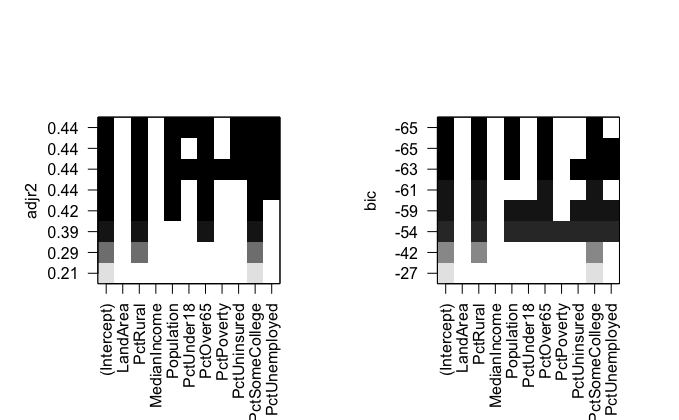
\includegraphics[width=3.8in]{bestsubsets} \\
      \end{center} 

      \begin{center}
        {Black indicates that a variable is included in the model, while white indicates that it is not.}
      \end{center} 
      
    \end{frame}


    \begin{frame}[fragile]{Putting things together}
      \begin{itemize}[<+->]
        \item Look at multiple statistics. They generally say similar things.
        \item Find the middle ground between an underspecified model and extraneous variables.
        \item Fine tune the model to get a correctly specified model - you may need to transform predictors and/or add interactions.
        \item Think about logical reasons why certain predictors might be useful, don't just focus on p-values.
      \end{itemize} 
    \end{frame}


    \begin{frame}[fragile]{Be careful of getting to crazy}
      \begin{itemize}[<+->]
        \item A general guideline is that you should not even consider more than one variable for every 10 to 15 cases in your dataset. 
        \item Otherwise, you can select the ones that happen to fit the data the best and essentially create a spurious correlation!
        \item Rember to check for multicolliearity and the LINE assumptions!
      \end{itemize} 
    \end{frame}


  \end{darkframes}
\end{document}
